% IEEE standard conference template; to be used with:
%   spconf.sty  - LaTeX style file, and
%   IEEEbib.bst - IEEE bibliography style file.
% --------------------------------------------------------------------------

\documentclass[letterpaper]{article}
\usepackage{spconf,amsmath,amssymb,graphicx}
\usepackage{booktabs}
\usepackage{float}

% Example definitions.
% --------------------
% nice symbols for real and complex numbers
\newcommand{\R}[0]{\mathbb{R}}
\newcommand{\C}[0]{\mathbb{C}}

% bold paragraph titles
\newcommand{\mypar}[1]{{\bf #1.}}

% Title.
% ------
\title{Bone Anisotropy Mapping}
%
% Single address.
% ---------------
\name{Jarunan Panyasantisuk, Joao Rivera, Rajan Gill, Ryan Cherifa } 
\address{Department of Computer Science\\ ETH Z\"urich\\Z\"urich, Switzerland}

% For example:
% ------------
%\address{School\\
%		 Department\\
%		 Address}
%
% Two addresses (uncomment and modify for two-address case).
% ----------------------------------------------------------
%\twoauthors
%  {A. Author-one, B. Author-two\sthanks{Thanks to XYZ agency for funding.}}
%		 {School A-B\\
%		 Department A-B\\
%		 Address A-B}
%  {C. Author-three, D. Author-four\sthanks{The fourth author performed the work
%		 while at ...}}
%		 {School C-D\\
%		 Department C-D\\
%		 Address C-D}
%

\begin{document}
%\ninept
%
\maketitle
%

The hard page limit is 6 pages in this style. Do not reduce font size
or use other tricks to squeeze. This pdf is formatted in the American letter format, so may look a bit strange when printed out.

\begin{abstract}
Describe in concise words what you do, why you do it (not necessarily
in this order), and the main result.  The abstract has to be
self-contained and readable for a person in the general area. You
should write the abstract last.
\end{abstract}

\section{Introduction}\label{sec:intro}

Bone fabric anisotropy or microstructure orientation was recently included in finite element (FE) models to improve the accuracy in predicting bone stiffness and strength. An FE model of bone is preferrably generated from a low resolution image which saves computing cost. Such a scanned image with a low resolution of 1-3mm can be obtained by widely-available clinical computer tomography (CT). However, the bone microstructure details can be obtained only by high resolution peripheral CT with the resolution of 60-82 $\mu$m. Bone anisotropy mapping methodology includes coordinates mapping between a low and a high-resolution images, region extraction, the mean intercept length (MIL) method for quantification of the microstructure orientation, ellipsoid fitting of MIL and eigendecomposition to obtain the major direction of the microstructure.

\mypar{Motivation} In the recent study, bone anisotropy mapping algorithms are performed for all low resolution image voxels and for all pairs (n=71) of low and high resolution images. This preprocessing step consumes a significant amount of computing time. Moreover, researchers expect larger dataset to create a more general FE models of bone. Therefore, the performance of these algorithms are crucial. Two software packages for image processing which include MIL calculation are Medtool, a commercialized PYTHON package, and BoneJ, an open-source JAVA plugin for ImageJ. The external packages needed to be integrated to the computation pipeline and optimization is not straightforward. 

In this paper, we are presenting an integrated and optimized methodology of bone anisotropy mapping. At our best knowledge, this is the first paper to optimize the performance of MIL calculation.
  
\section{Background}\label{sec:background}
% Coord mapping & region extraction
The methodology is shown in Fig.~\ref{fig:method}. Coordinates from a low resolution image were mapped to its own high resolution image. Then, a sphere region is extracted and centered at the mapped coordinate in the high reoslution image. 
% MIL
Subsequently, the anisotropy of the extracted bone region is quantified by using the mean intercept length (MIL) method which imposed direction vectors on the regions. The mean length of each vector is the sum of the length inside the bone region devided by the number of intercepts which intersect with bone/non-bone transition.
% ellipsoid fitting
The MIL values can be plots as a cloud of points in the direction vector space and an ellipsoid can be fitted to obtain a representative two dimensional tensor, for which three eigenvalues and three eigenvectors are calculated. The eigenvector associated with the minimum eigenvalue is the major direction of that bone region.

\begin{figure}[ht]
  \centering
  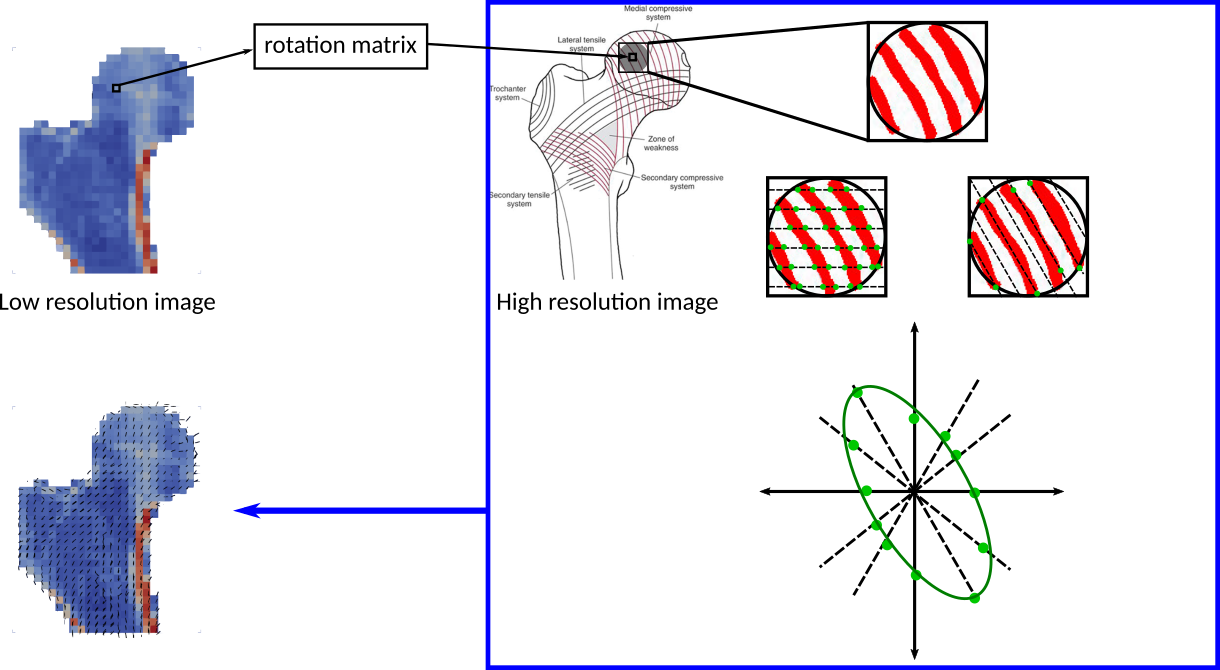
\includegraphics[width=3.5in]{figs/overview.png}
  \caption{Methodology}
  \label{fig:method}
\end{figure}


\mypar{Region extraction}
Applying mask on the bone region requires a multiplication for each image voxel.

\mypar{Mean Intercept Length (MIL) method}

% todo: add figure of MIL 
The mean intercept length of the vector $v$ can be expressed as:
\begin{equation}
  MIL(v) = \frac{h}{C(v)}
\end{equation}
where $h$ is the summation of the length of all direction vectors and $C(v)$ is the number of intercepts of the vector $v$.
The algorithm includes an addition and a comparison. 

% todo: algorithm for ellipsoid fitting
\mypar{Ellipsoid fitting} algorithm ...

\begin{table}
  \caption{Cost analysis}
  \begin{tabular}{l c c c}
    \toprule
     & flops & read/write & Operational intensity\\
     &   & [doubles] & [flops/double]\\
    \midrule
    Region extractions & $n^{3}$ & $3n^{3}$ & 1/3\\
    MIL \\
    Ellipsoid fitting\\
    \bottomrule
  \end{tabular}
\end{table}




\section{Methods}\label{sec:yourmethod}

% todo: 
% - basic implementation, quantify the perentage of each algorithm takes.
% - testing machine


\mypar{Region extraction} Loop unrolling


\mypar{MIL} Loop unrolling and scalar replacement, blocking, SIMD blocking.

\mypar{Ellipsoid fitting} moving loop invariant code, SIMD


\section{Experimental Results}\label{sec:exp}

Here you evaluate your work using experiments. You start again with a
very short summary of the section. The typical structure follows.

\mypar{Experimental setup} Specify the platform (processor, frequency, cache sizes)
as well as the compiler, version, and flags used. I strongly recommend that you play with optimization flags and consider also icc for additional potential speedup.

Then explain what input you used and what range of sizes. The idea is to give enough information so the experiments are reproducible by somebody else on his or her code.

\mypar{Results}
\begin{figure}[H]
  \centering
 
  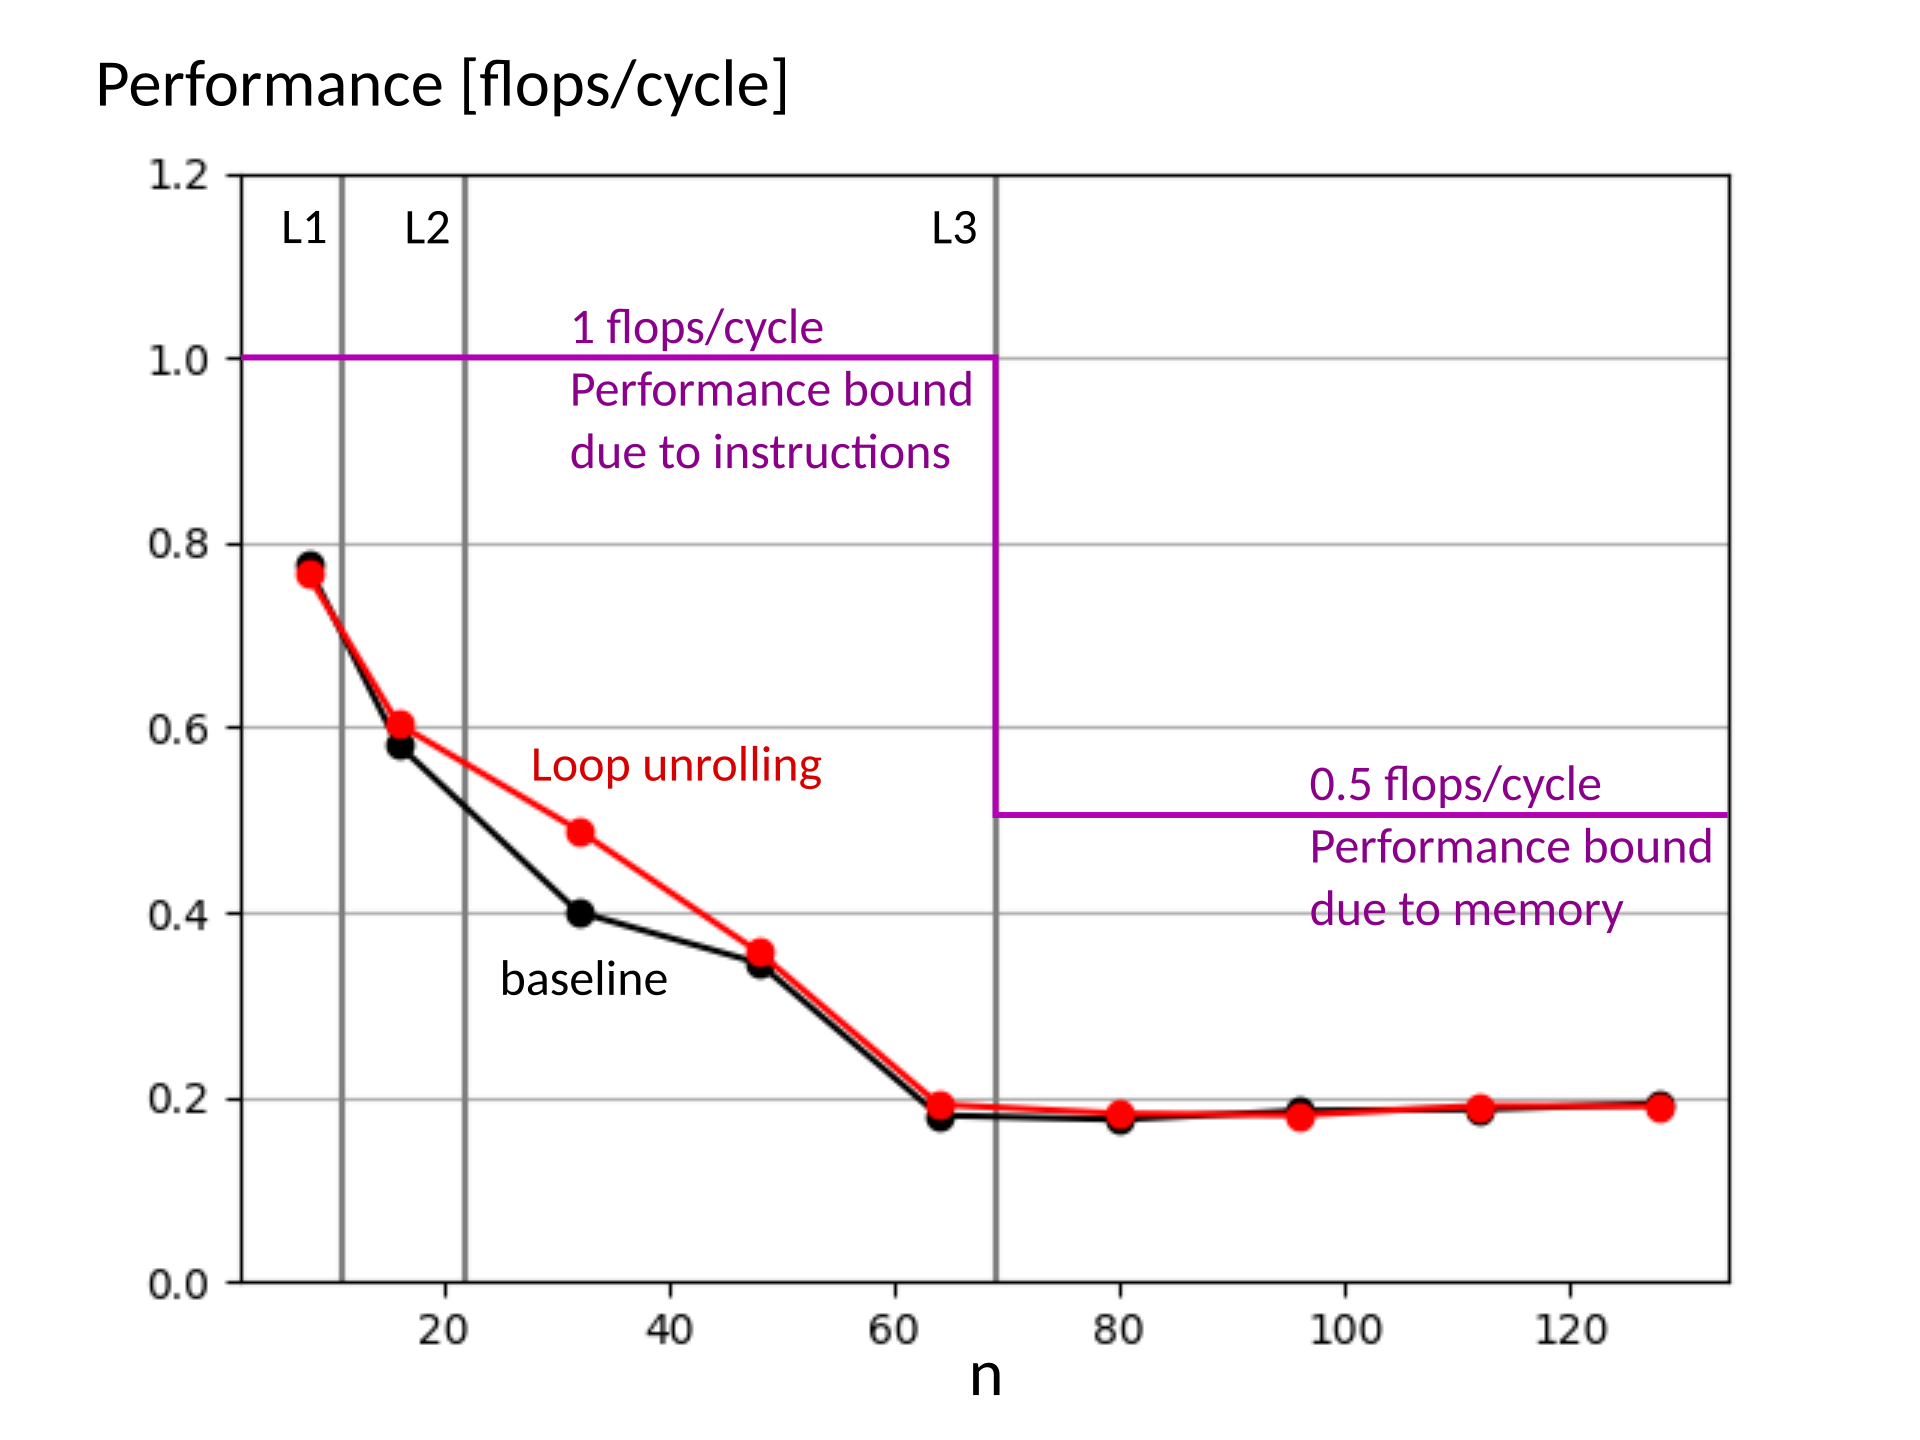
\includegraphics[width=3.5in]{figs/plots/regions/regions_performance_labelled.png}
  \caption{Performance of region extraction}
  \label{res:regions}
\end{figure}

\begin{figure}[H]
  \centering
  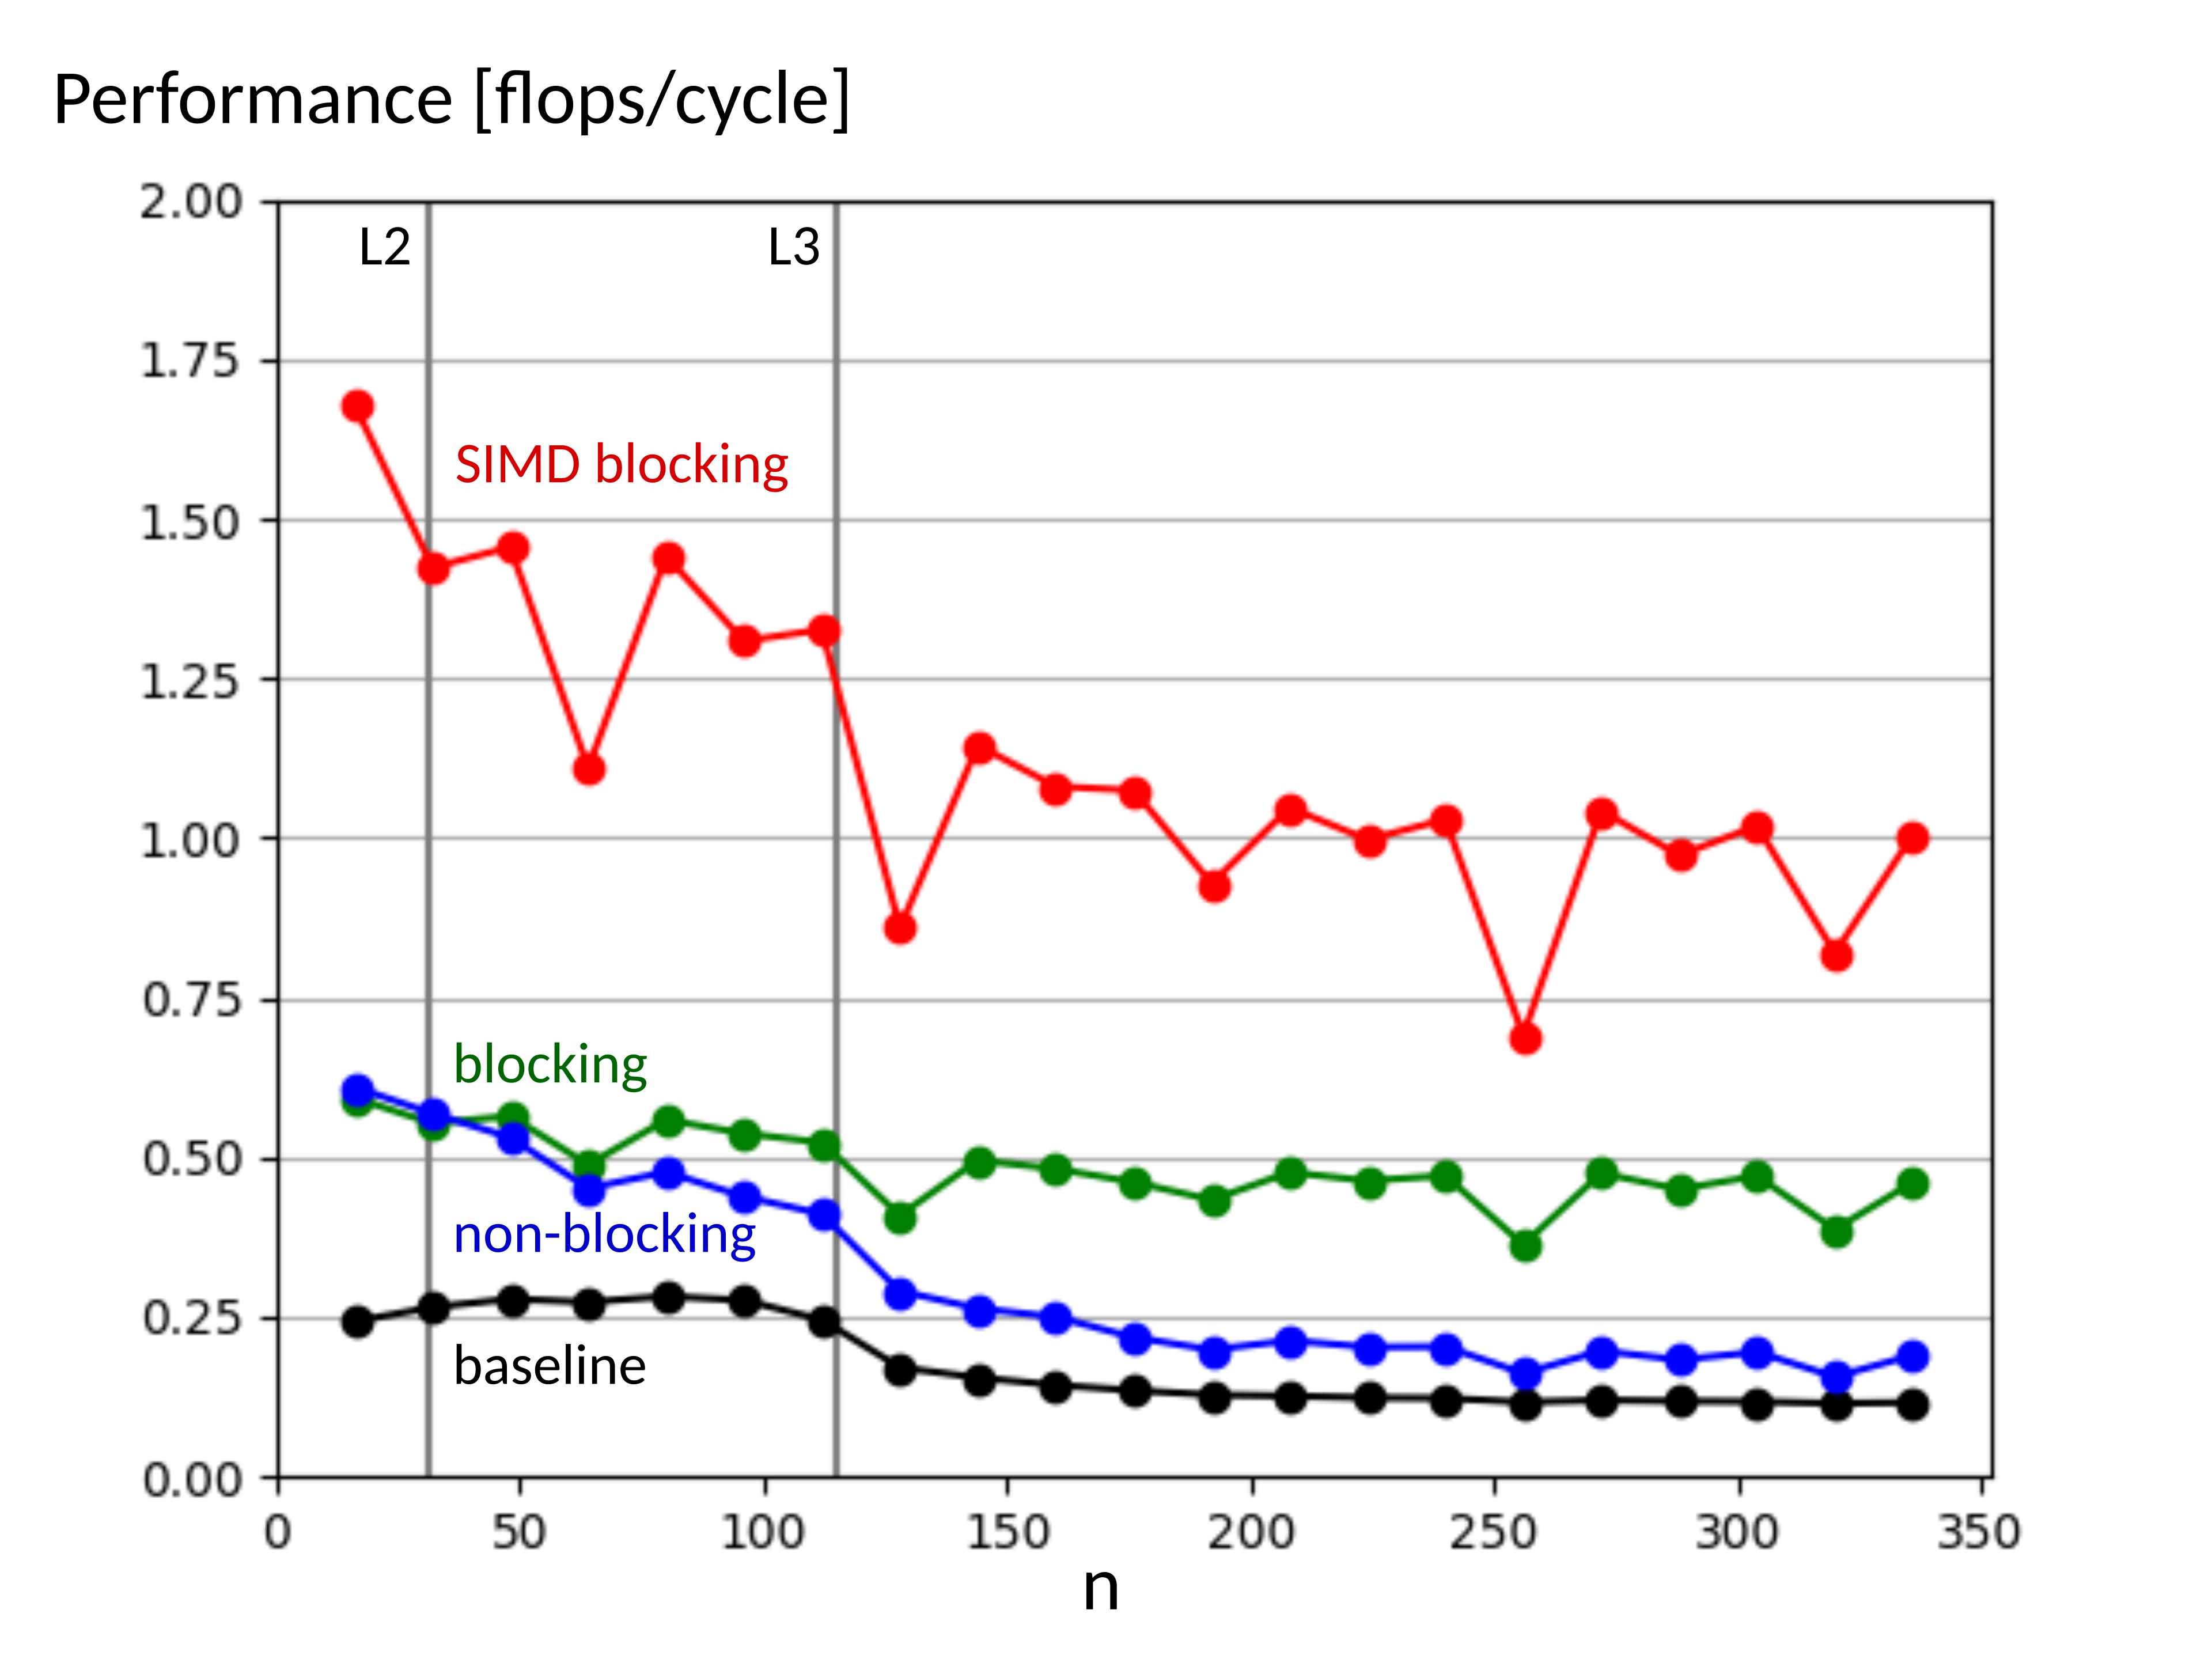
\includegraphics[width=3.5in]{figs/plots/mil/mil_performance_labelled.png}
  \caption{Performance of MIL}
  \label{res:mil}
\end{figure}


\begin{figure}[H]
  \centering
  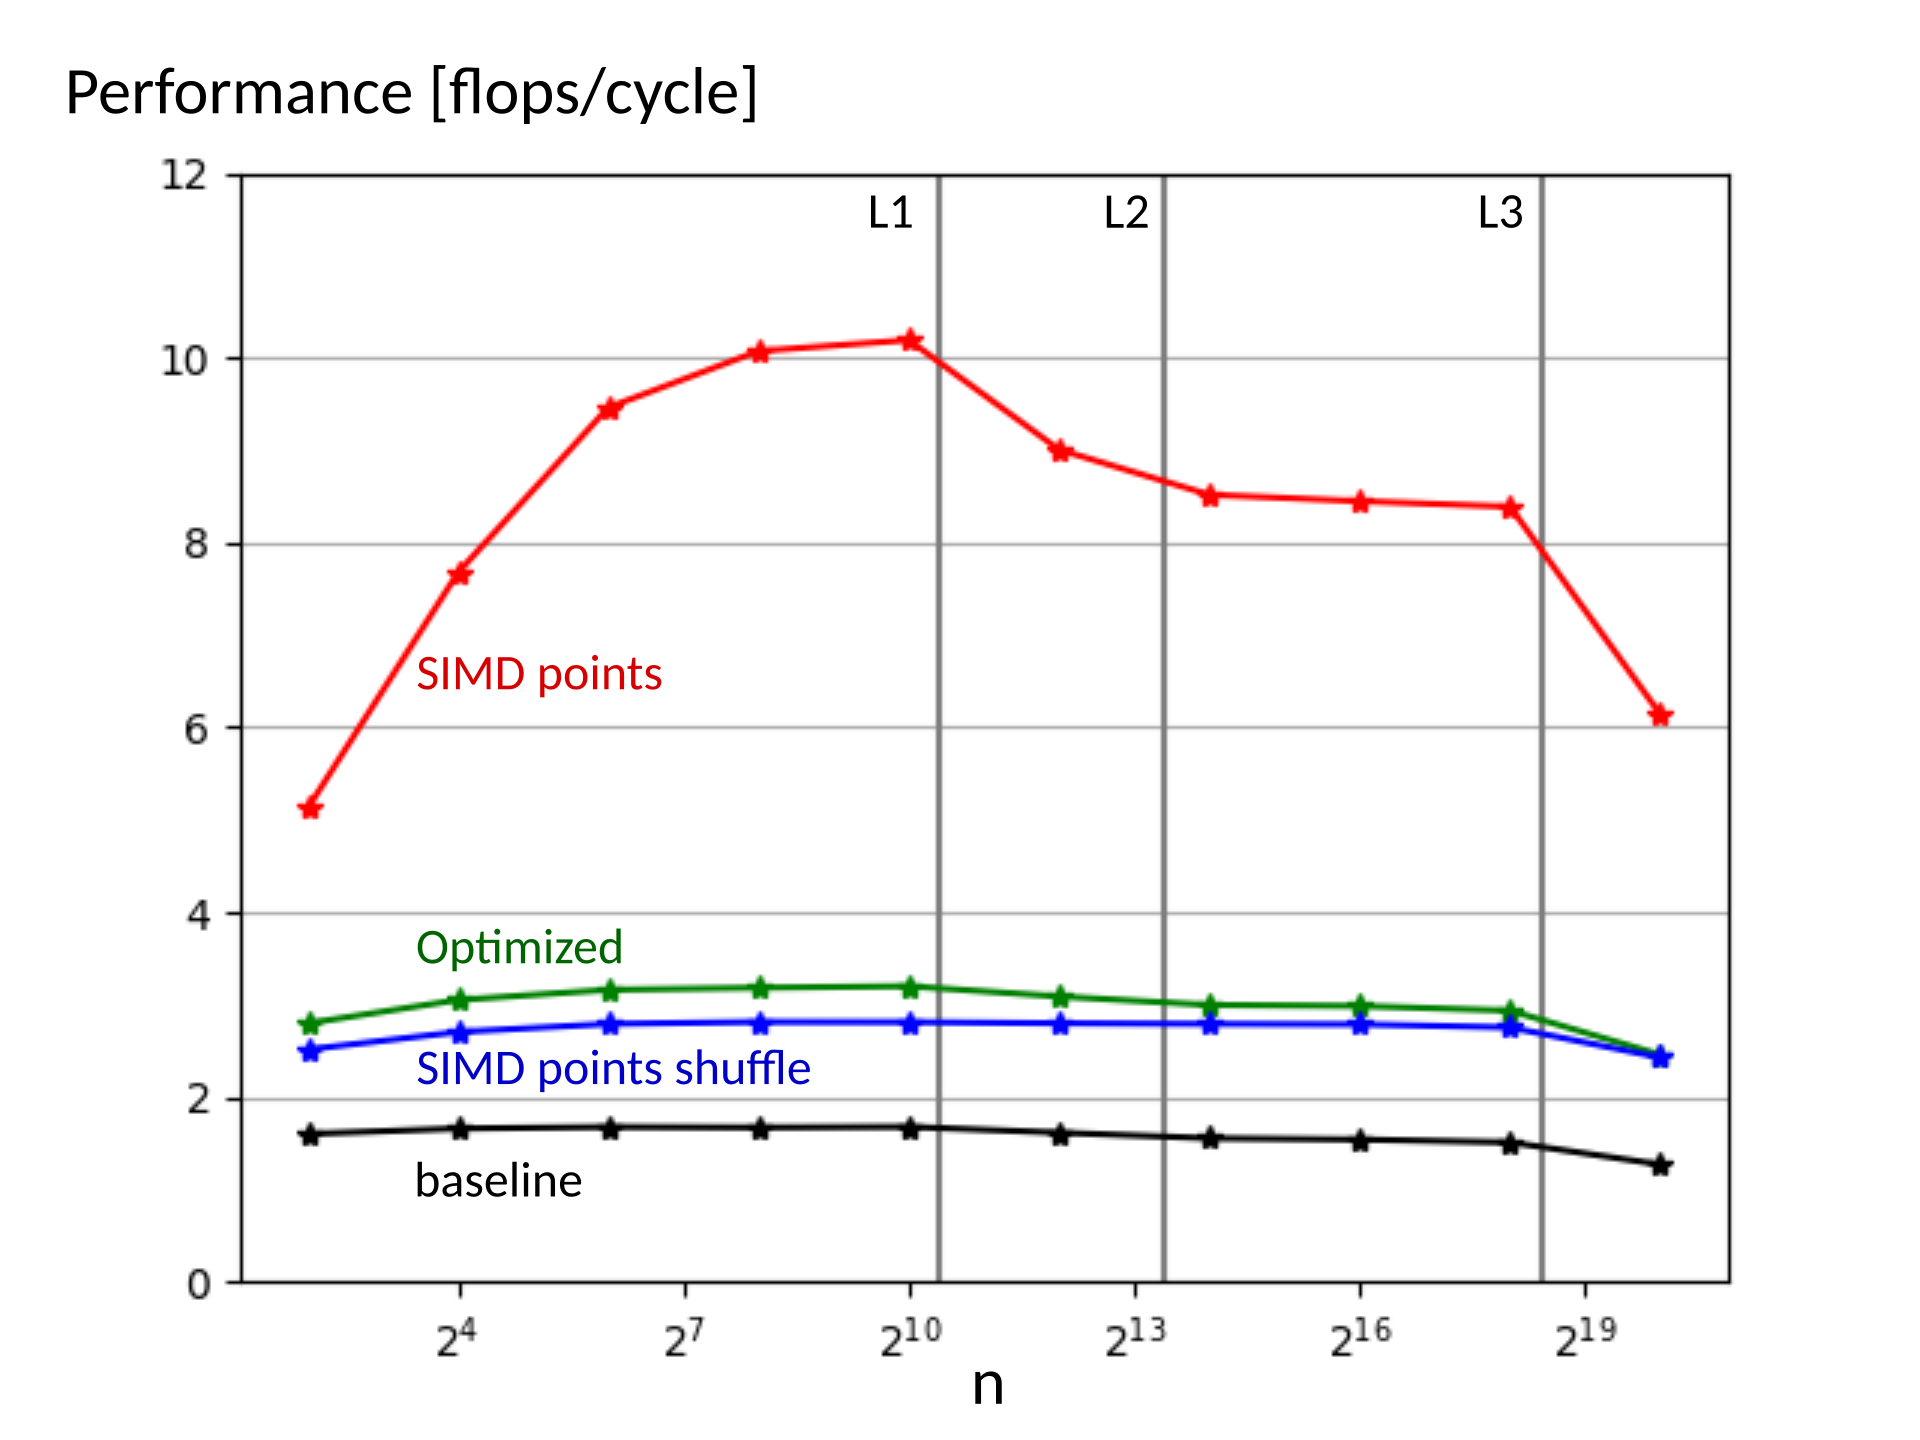
\includegraphics[width=3.5in]{figs/plots/ellipsoid/ellipsoid_performance_labelled.png}
  \caption{Performance of ellipsoid}
  \label{res:ellipsoid}
\end{figure}


\section{Conclusions}

Here you need to briefly summarize what you did and why this is
important. {\em Do not take the abstract} and put it in the past
tense. Remember, now the reader has (hopefully) read the paper, so it
is a very different situation from the abstract. Try to highlight
important results and say the things you really want to get across
(e.g., the results show that we are within 2x of the optimal performance ... 
Even though we only considered the DFT, our optimization
techniques should be also applicable ....) You can also formulate next
steps if you want. Be brief.

\section{Further comments}

Here we provide some further tips.

\mypar{Further general guidelines}

\begin{itemize}
\item For short papers, to save space, I use paragraph titles instead of
subsections, as shown in the introduction.

\item It is generally a good idea to break sections into such smaller
units for readability and since it helps you to (visually) structure the story.

\item The above section titles should be adapted to more precisely
reflect what you do.

\item Each section should be started with a very
short summary of what the reader can expect in this section. Nothing
more awkward as when the story starts and one does not know what the
direction is or the goal.

\item Make sure you define every acronym you use, no matter how
convinced you are the reader knows it.

\item Always spell-check before you submit (to me in this case).

\item Be picky. When writing a paper you should always strive for very
high quality. Many people may read it and the quality makes a big difference.
In this class, the quality is part of the grade.

\item Books helping you to write better: \cite{Higham:98} and \cite{Strunk:00}.

\item Conversion to pdf (latex users only): 

dvips -o conference.ps -t letter -Ppdf -G0 conference.dvi

and then

ps2pdf conference.ps
\end{itemize}

\mypar{Graphics} For plots that are not images {\em never} generate (even as intermediate step)
jpeg, gif, bmp, tif. Use eps, which means encapsulate postscript, os pdf. This way it is
scalable since it is a vector graphic description of your graph. E.g.,
from Matlab, you can export to eps or pdf.

Here is an example of how to get a plot into latex
(Fig.~\ref{fftperf}). Note that the text should not be any smaller than shown.

\begin{figure}\centering
  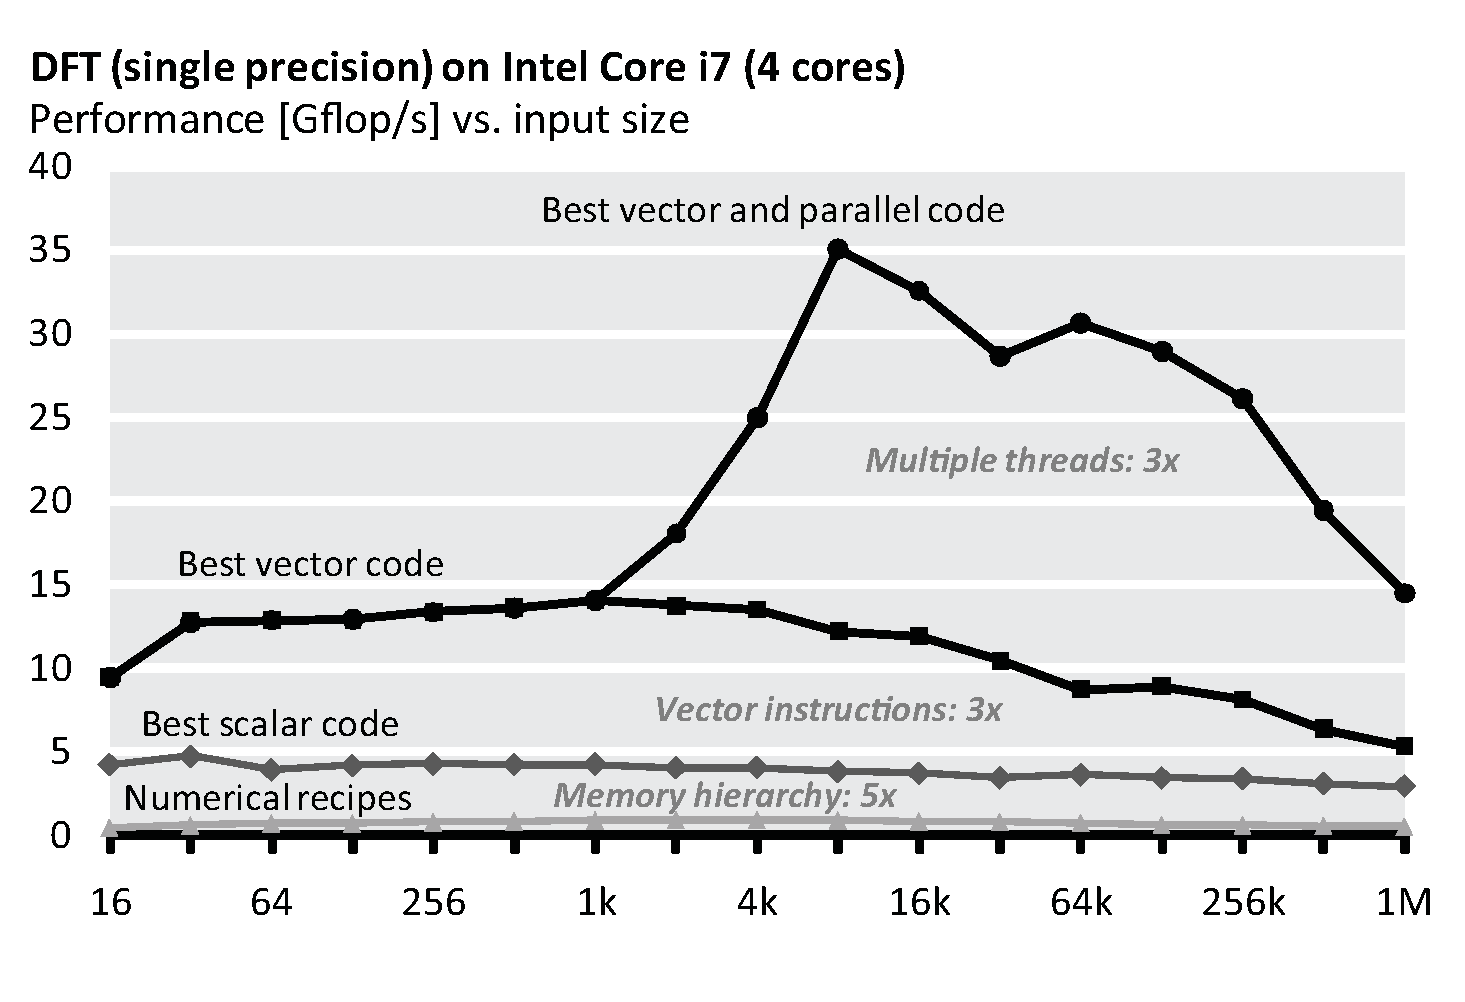
\includegraphics[scale=0.33]{dft-performance.eps}
  \caption{Performance of four single precision implementations of the
  discrete Fourier transform. The operations count is roughly the
  same. {\em The labels in this plot are too small.}\label{fftperf}}
\end{figure}



% References should be produced using the bibtex program from suitable
% BiBTeX files (here: bibl_conf). The IEEEbib.bst bibliography
% style file from IEEE produces unsorted bibliography list.
% -------------------------------------------------------------------------
\bibliographystyle{IEEEbib}
\bibliography{bibl_conf}

\end{document}

